\usepackage{environ}

\newcommand{\sepframe}[2]{
    \setbeamercolor{background canvas}{bg=afupbluebackground}

    \begin{frame}[noframenumbering,plain]
        \begin{tikzpicture}[remember picture,overlay]
            \fill[afuppink] (0,0) rectangle(.05,\paperheight);
        \end{tikzpicture}
      \begin{tikzpicture}[remember picture,overlay]
          \ifx\insertframesubtitle\@empty%
              {\node[anchor=west, afupblue, font=\huge] at (0,.25){\uppercase\expandafter{#1}};}
          \else%
              {
                  \node[anchor= west, afupblue, font=\huge] at (0,.25){\uppercase\expandafter{#1}};%
                  \node[anchor= west, afuppink,font=\small] at (0,-.5){\uppercase\expandafter{#2}};}%
          \fi
      \end{tikzpicture}

      \begin{tikzpicture}[remember picture, overlay]
          \node at (current page.south east) {
              
\includegraphics[trim=0 -4cm -4cm 0, scale=.35, keepaspectratio]{src/afup/style/logo/afup-icon-color}
            };
      \end{tikzpicture}
    \end{frame}
  }

\NewEnviron{sepFrameA}[3][]{%
    \begin{frame}
        \begin{columns}
            \column{\paperwidth}
                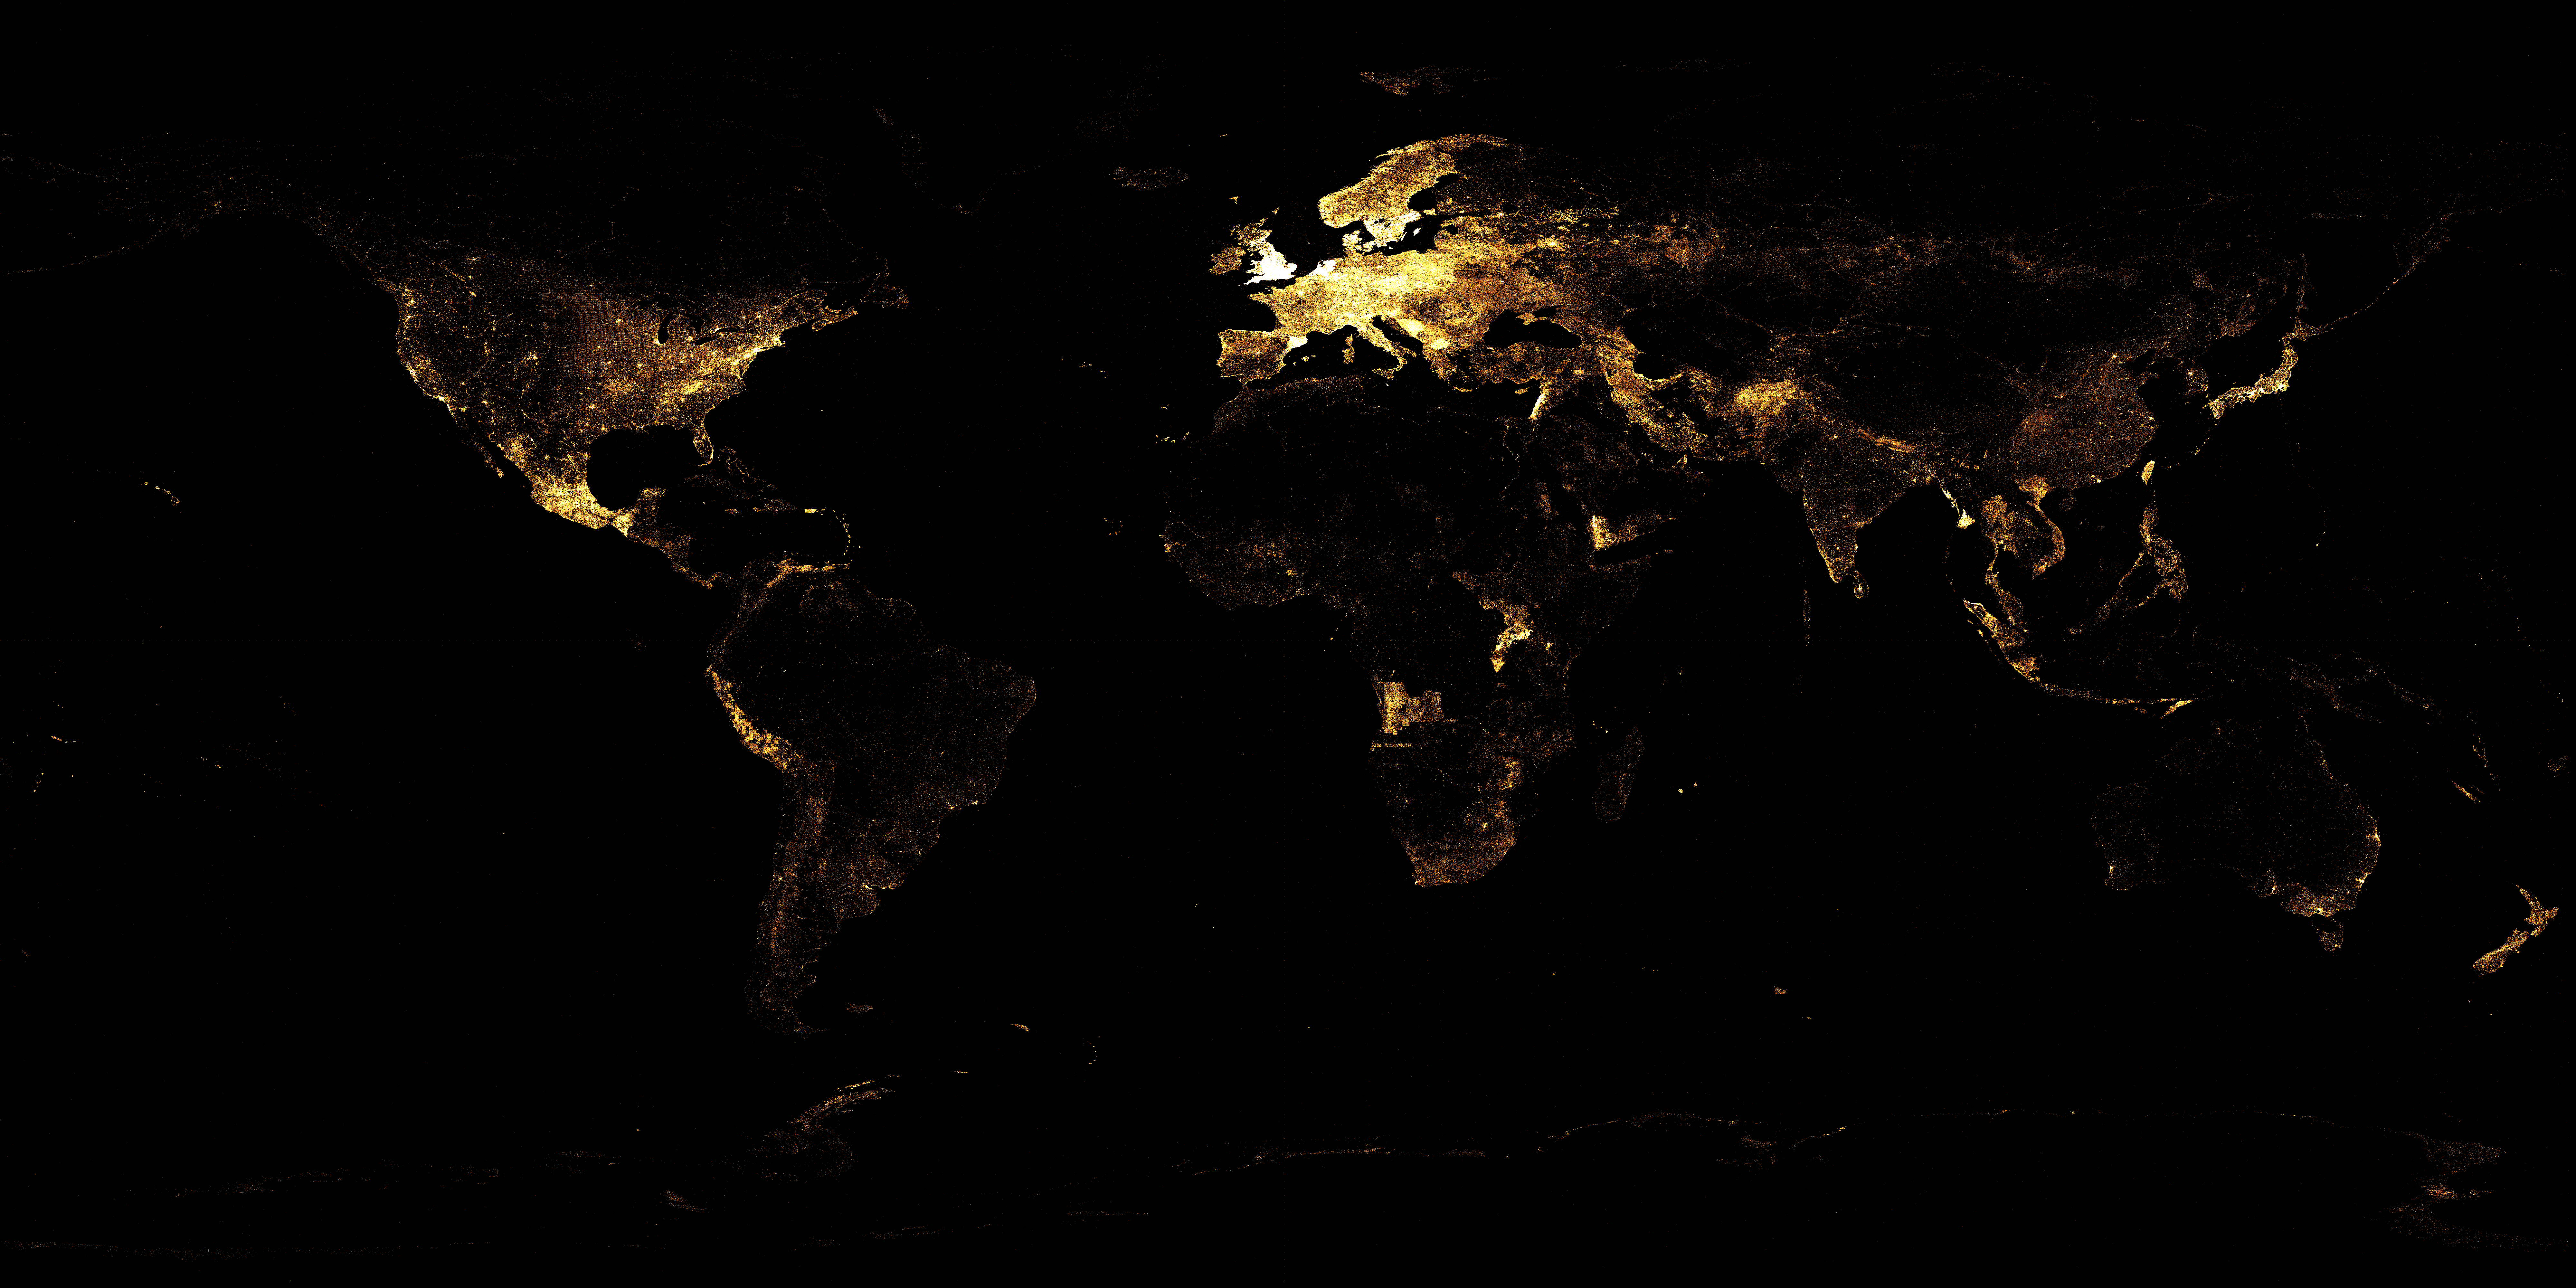
\includegraphics[width=\the\paperwidth, height=.5\paperheight]{src/afup/style/logo/bg1}
            \begin{tikzpicture}
                \node[shape=rectangle, text opacity=1,minimum height=.5\paperheight, minimum width=\paperwidth, anchor=south]{
                    \BODY
                };
            \end{tikzpicture}
          \end{columns}
    \end{frame}
}

\NewEnviron{sepFrameB}[3][]{%
    \begin{frame}
        \begin{columns}
            \column{.5\paperwidth}
                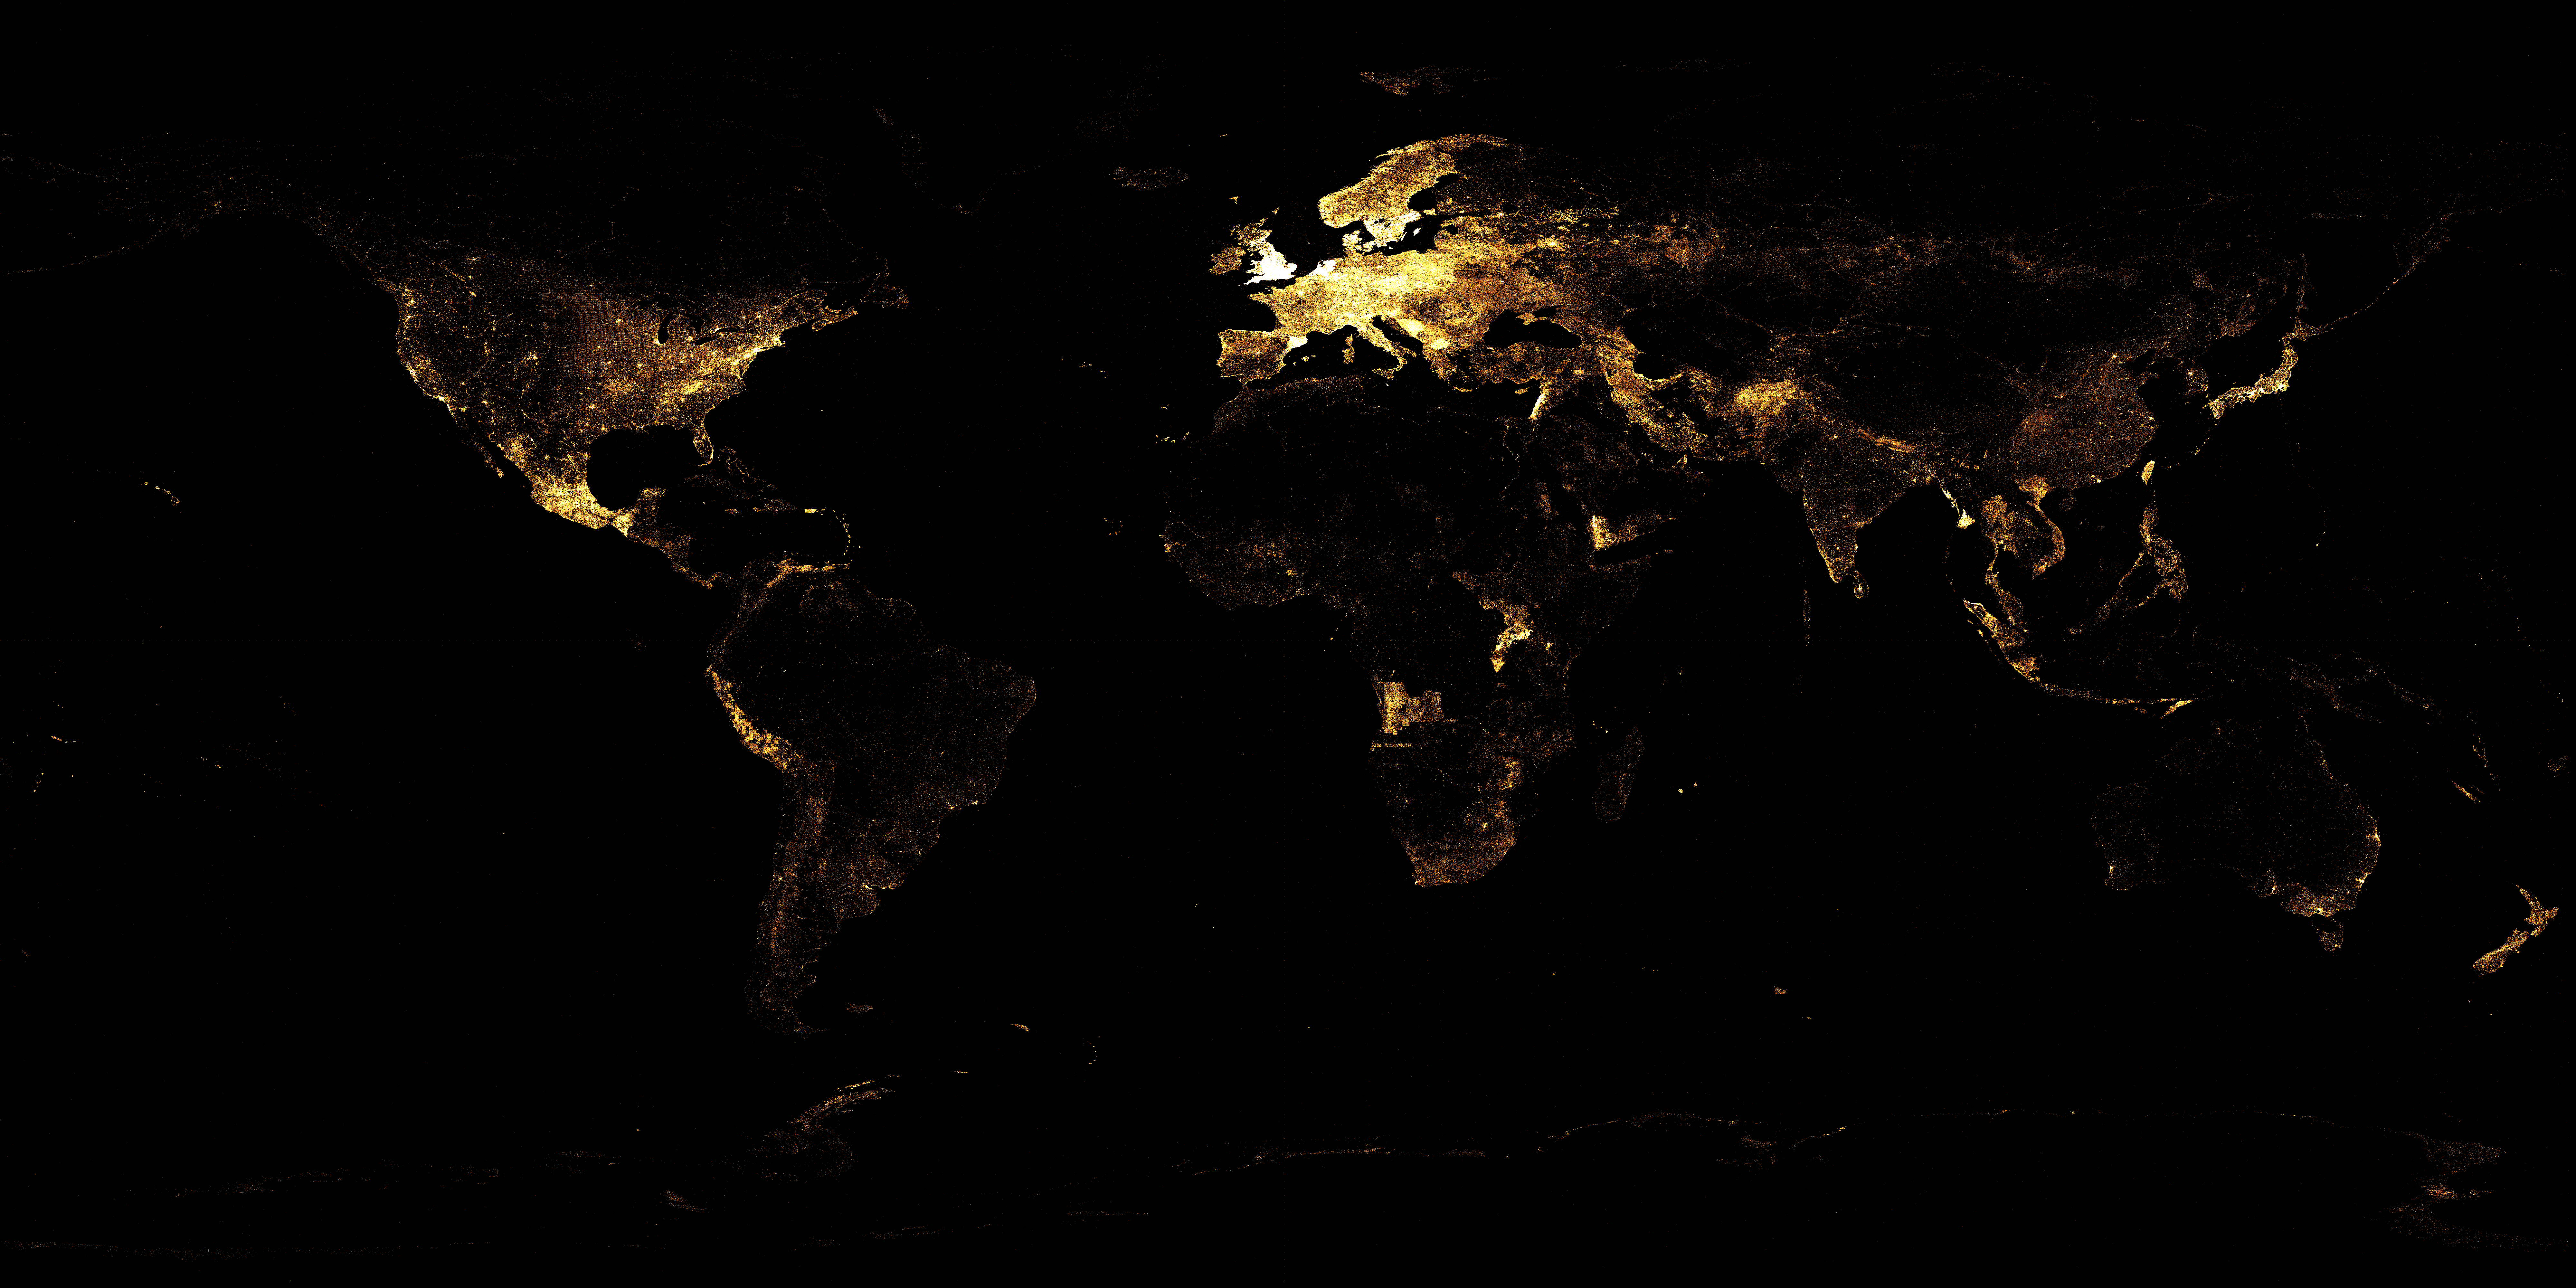
\includegraphics[width=.5\paperwidth, height=\paperheight]{src/afup/style/logo/bg1}
            \column{.5\paperwidth}
                \begin{tikzpicture}
                    \node[shape=rectangle, text opacity=1,minimum height=\paperheight, minimum width=.5\paperwidth, anchor=east]{
                        \BODY
                    };
                \end{tikzpicture}
        \end{columns}
    \end{frame}
}


% To read: https://tex.stackexchange.com/questions/113410/removing-sidebar-from-a-single-beamer-frame
% To read: https://github.com/deuslirio/UFGTeX-Presentation
% To read: https://github.com/matze/mtheme
